% ============================================================
%  Section 5.3: Results — Scaling Study
%  H&E to Sirius Red Virtual Staining Paper
% ============================================================

\subsection{Results: Scaling Study}
\label{sec:results_scaling}

Quantitative results for all 54 configurations are shown in
Figure~\ref{fig:results_overview}, which plots all four metrics jointly across the
full experiment.
Each point corresponds to one configuration; colour encodes data fraction and marker
shape encodes generator size.
Four high-level patterns emerge: (i)~CPA~MAE spans over an order of magnitude
($0.008$--$0.171$) and is far more discriminative than the perceptual metrics, which
saturate within a narrow band for well-behaved GAN configurations; (ii)~CycleDiffusion
attains systematically lower Patch-SSIM ($0.200$--$0.293$) than GAN-based methods
($0.298$--$0.349$), irrespective of scale; (iii)~two model families exhibit training
instability under specific scaling conditions; and (iv)~perceptual metric rankings
correlate only moderately with the CPA~MAE ranking.

\begin{figure*}[t!]
  \centering
  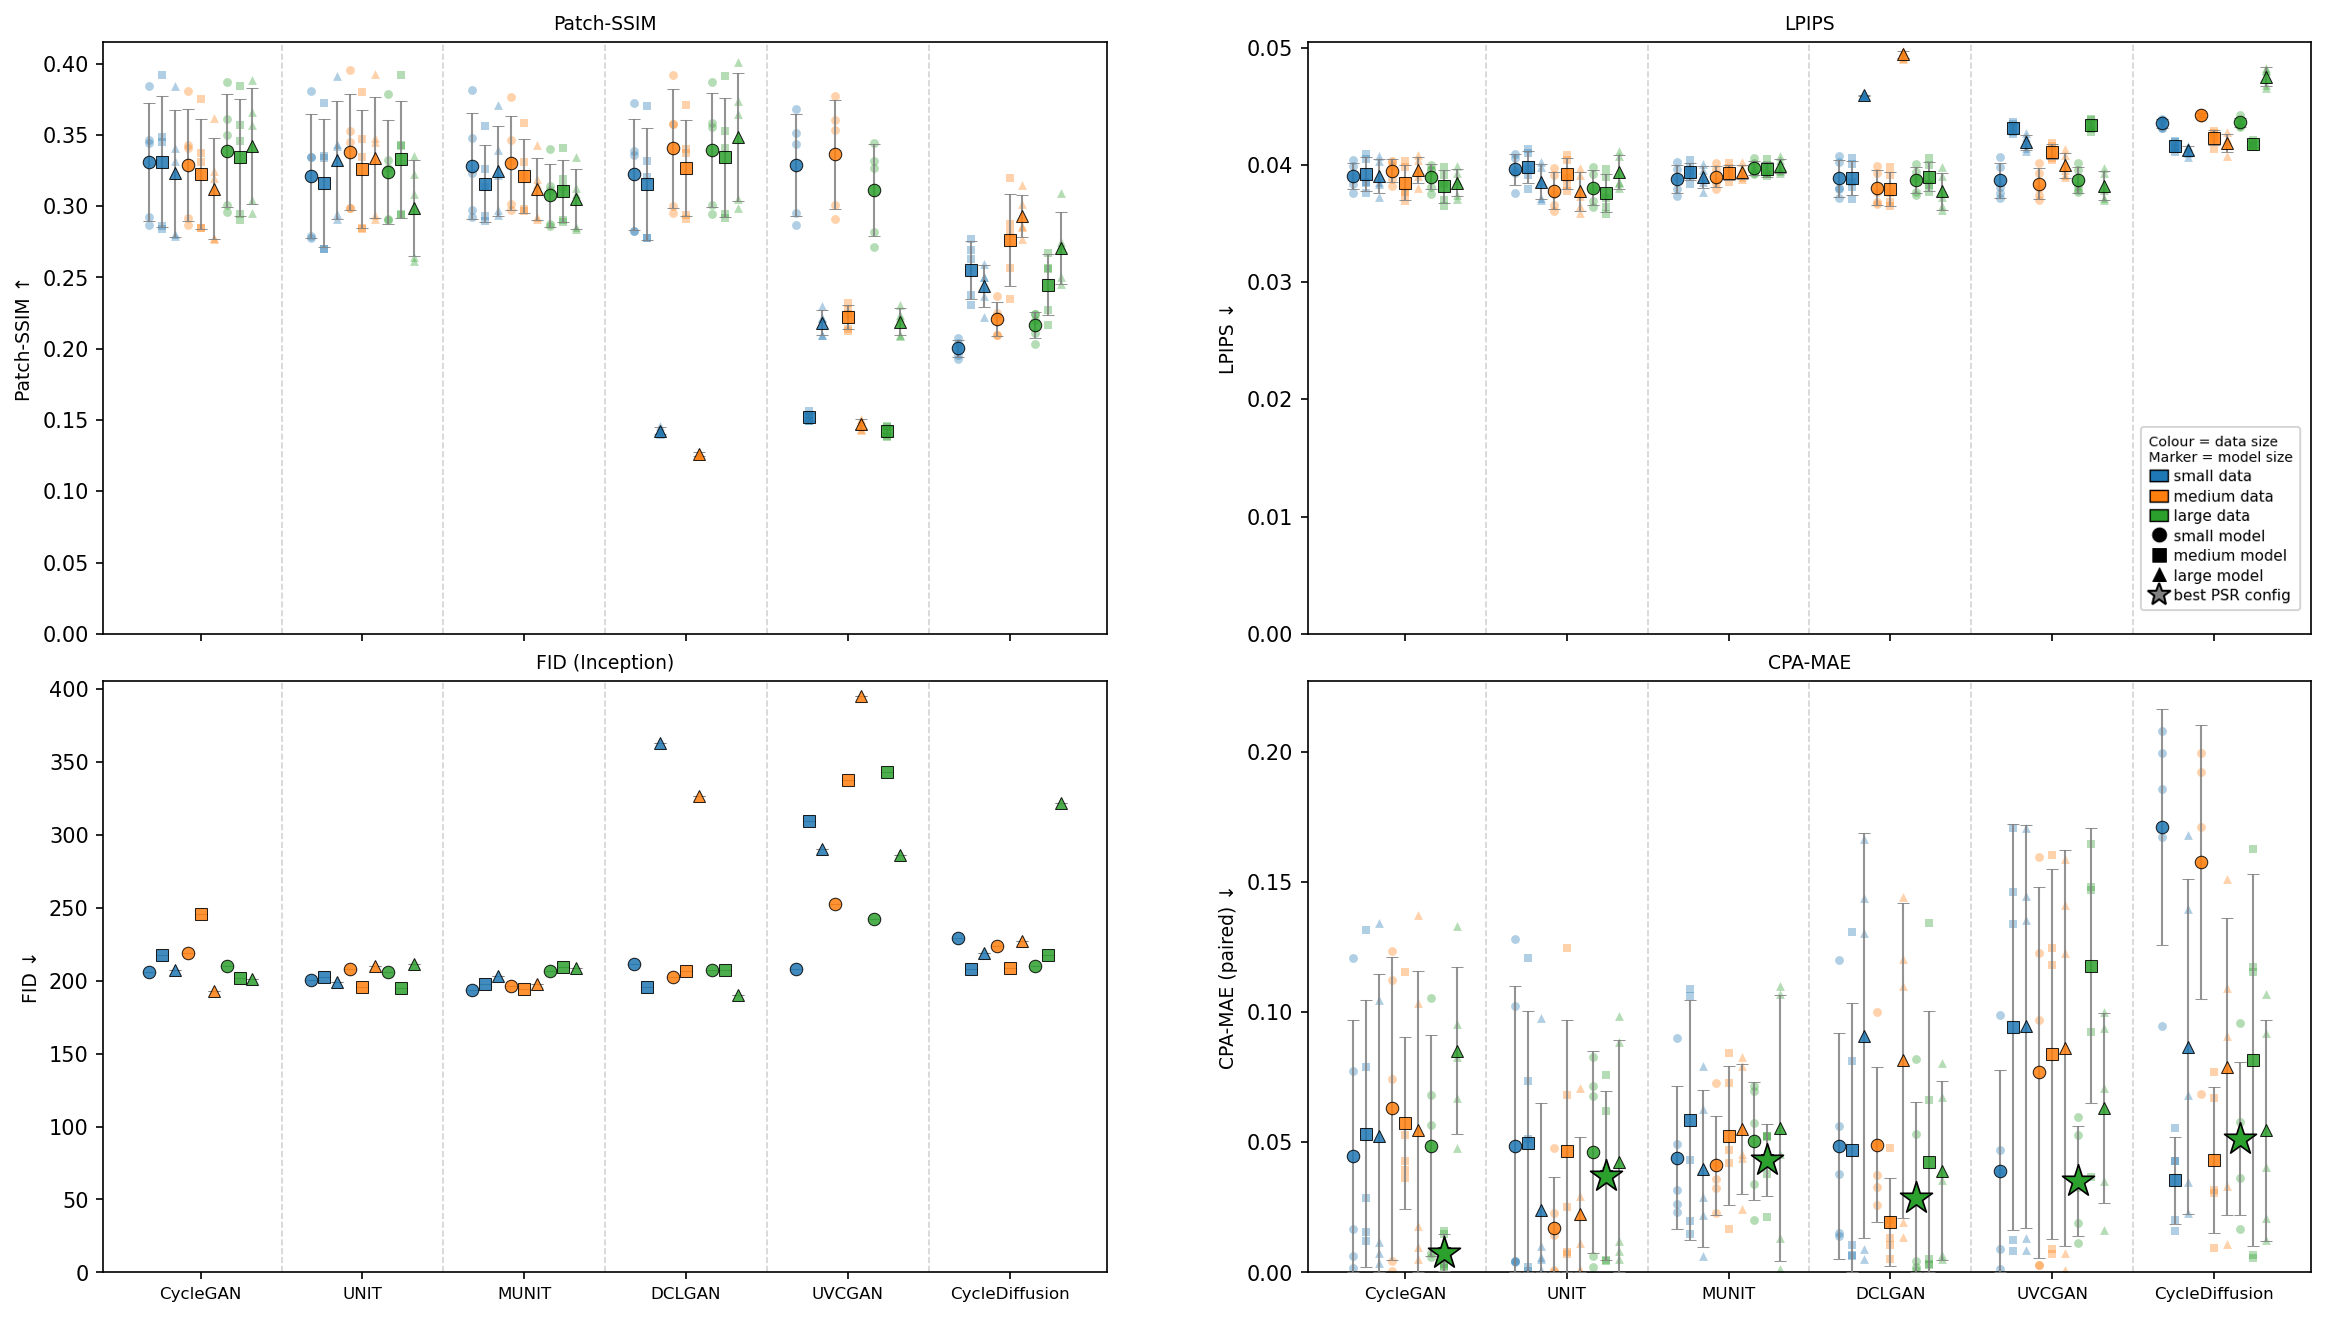
\includegraphics[width=\linewidth]{images/combined_metrics}
  \caption{%
    All four evaluation metrics across the 54 scaling configurations
    ($6~\text{models} \times 3~\text{sizes} \times 3~\text{data fractions}$).
    Colour encodes training data fraction (blue: 25\%, orange: 50\%, green: 100\%);
    marker shape encodes generator size (circle: small, square: medium, triangle: large).
    Large star markers indicate the best-performing model size at the 100\% data fraction
    per model family, selected for ensemble uncertainty estimation in
    Section~\ref{sec:uncertainty}.
    Error bars on Patch-SSIM, LPIPS, and CPA~MAE denote $\pm$\,std over $N{=}5$ test
    WSIs; FID is a set-level statistic with no per-sample variance.
    Vertical axis directions: Patch-SSIM higher is better; LPIPS, FID, CPA~MAE lower
    is better.%
  }
  \label{fig:results_overview}
\end{figure*}

% -------------------------------------------------------

Per-family results across the full size~$\times$~data-fraction grid are summarised
below; complete metric tables for all 54 configurations are in Supplementary Sec.~6.

\textbf{CycleGAN:}
Patch-SSIM ($0.312$--$0.342$) and LPIPS ($0.038$--$0.040$) are near-invariant across
all nine configurations; FID ($193$--$245$) shows no monotonic size trend.
CPA~MAE is the most discriminative axis: at 100\% data, small/medium/large yield
$0.049$/$0.008$/$0.085$, with the medium generator achieving the lowest CPA~MAE in the
entire study ($0.008 \pm 0.007$).
Across data fractions, perceptual metrics are insensitive to data volume while CPA~MAE
shows no consistent trend for any generator size.

\textbf{UNIT:}
Perceptual metrics (Patch-SSIM $0.298$--$0.338$, LPIPS $0.037$--$0.040$, FID
$195$--$211$) are stable across the full grid.
CPA~MAE at 100\% data is $0.046$/$0.037$/$0.043$ (S/M/L), with no consistent size
advantage; the small generator achieves its best CPA~MAE at 50\% data ($0.017$) rather
than 100\%.

\textbf{MUNIT:}
The most stable family: all four metrics span narrow ranges across all nine cells
(Patch-SSIM $0.305$--$0.331$, LPIPS $0.039$--$0.040$, FID $193$--$210$, CPA~MAE
$0.040$--$0.059$), with no generator size or data fraction yielding a systematic
advantage.

\textbf{DCLGAN:}
At 100\% data all three sizes are stable (CPA~MAE $0.028$--$0.042$, FID $190$--$212$);
the large generator achieves the study-best FID ($190.0$).
At 50\% and 25\% data, the large generator collapses~(Patch-SSIM $0.126$--$0.143$, FID
$327$--$363$, CPA~MAE $0.082$--$0.091$), while small and medium sizes remain stable
(CPA~MAE $0.019$--$0.049$) at all data fractions.

\textbf{UVCGAN:}
The small generator is stable across all data fractions (Patch-SSIM $0.311$--$0.337$,
CPA~MAE $0.035$--$0.077$).
Medium and large variants are degraded across all data fractions (Patch-SSIM
$0.142$--$0.222$, FID $286$--$395$, CPA~MAE $0.063$--$0.118$), with the medium
generator reaching its highest CPA~MAE at 100\% data ($0.118 \pm 0.053$).

\textbf{CycleDiffusion:}
Consistently lower Patch-SSIM ($0.200$--$0.293$) and higher LPIPS ($0.041$--$0.048$)
than all GAN-based families, reflecting the DDIM inversion inductive bias.
At 100\% data, CPA~MAE is $0.051$/$0.082$/$0.055$ (S/M/L); the small generator's
CPA~MAE rises sharply with data reduction (exceeding $0.15$ at both 50\% and 25\% data,
reaching $0.171$ at 25\%), while the medium generator achieves its lowest CPA~MAE at
25\% data ($0.035$) rather than at 100\% ($0.082$).


% -------------------------------------------------------

\begin{table}[h!]
  \centering
  \caption{Spearman rank correlation ($r_s$) between the four metric orderings over
    all 54 configurations (rank~1 = best per metric). All off-diagonal values
    significant at $p{<}0.001$.}
  \label{tab:ranking_correlation}
  \begin{tabular}{lcccc}
    \toprule
     & Patch-SSIM & LPIPS & FID & CPA~MAE \\
    \midrule
    Patch-SSIM & 1.00 & & & \\
    LPIPS      & 0.82 & 1.00 & & \\
    FID        & 0.60 & 0.49 & 1.00 & \\
    CPA~MAE    & 0.63 & 0.64 & 0.55 & 1.00 \\
    \bottomrule
  \end{tabular}
\end{table}

\textbf{Metric agreement:}
Table~\ref{tab:ranking_correlation} shows Spearman rank correlations between the four
metric orderings over all 54 configurations (rank~1 assigned to the best-performing
configuration per metric; all pairs significant at $p{<}0.001$).
Patch-SSIM and LPIPS rankings agree most strongly with each other ($r_s{=}0.82$).
FID shows only moderate agreement with both Patch-SSIM ($r_s{=}0.60$) and LPIPS
($r_s{=}0.49$).
CPA~MAE likewise shows only moderate agreement with all three perceptual metrics:
$r_s{=}0.63$ with Patch-SSIM, $r_s{=}0.64$ with LPIPS, and $r_s{=}0.55$ with FID.
